\documentclass[12pt]{article}
\usepackage[utf8]{inputenc}
\usepackage{footmisc}
\usepackage[margin=1in]{geometry}
\usepackage{graphicx}
\usepackage{listings}
\usepackage{float}
\usepackage{xcolor}
\usepackage[
backend=biber,
style=alphabetic,
]{biblatex}
\usepackage{fancyhdr}               % custom header/footer
\definecolor{backcolour}{rgb}{0.95,0.95,0.92}
\definecolor{codegreen}{rgb}{0,0.6,0}
\definecolor{codegray}{rgb}{0.5,0.5,0.5}
\definecolor{codepurple}{rgb}{0.58,0,0.82}
\lstdefinestyle{mystyle}{
    backgroundcolor=\color{backcolour},
        commentstyle=\color{codegreen},
    keywordstyle=\color{magenta},
    numberstyle=\tiny\color{codegray},
    basicstyle=\ttfamily\footnotesize,
    numbers=left,                    
    numbersep=5pt, 
}

\lstset{style=mystyle}

\pagestyle{fancy}
\fancyhf{}
\cfoot{\thepage}
\lhead{Brasen, Tenorio}
\rhead{Arizona Real Estate Analysis}
\setlength{\headheight}{15pt}

\addbibresource{citations.bib}

\begin{document}
\title{MAT 494\\Arizona Housing Market Analysis}

\author{
Dean Brasen\thanks{dsbrasen@asu.edu}, 
Joshua Tenorio\thanks{jltenori@asu.edu}
}
\date{November 20, 2022}
\maketitle
\begin{abstract}
    {\bf Keywords:} Arizona housing; Arizona real estate.
\end{abstract}
\tableofcontents
\section{Introduction}
In this paper, we will be taking real estate data from Arizona data to make models predicting future outcomes.
This will involve the use of neural networks and data extrapolation in Python.
\vspace{1em}


Motivation: Housing price loans have dramatically increased throughout 2022. For instance according to Lieb, rent is nearly 30\% higher in Arizona than in 2021 \cite{lieb-rent}, and the housing GDP in the US has gone down around 1\% \cite{hammond-GDP}. Being able to understand and predict this for the future would have a wide range of uses to prevent further damage to the economy especially as Arizona and the metro Phoenix area continues to grow.
\section{Data Description}
The Kaggle dataset we will be using is titled Arizona Houses 2021, and was uploaded by Antonio N \cite{kaggle-set}.
It is licensed in the public domain with the CC0 license, and has a usability score of 8.24.
It has 563 data points and 8 columns:
\begin{enumerate}
    \item Price
    \item Address
    \item Local Area
    \item Zipcode
    \item Number of beds
    \item Number of baths
    \item Square footage of the house
    \item URL
\end{enumerate}

For this project, our dependent variable was the price.
Although the dataset included a URL to Zillow, this column was not used for our purposes.

\subsection{Additional Features}
Additional features were added in order to better use the dataset.
In order to effectively use k-means, GPS coordinates of each zip code was added.
With positioning data available for use, we used k-means to categorizes houses as either North AZ, Central AZ, and South AZ.

Another feature added was the city index.
This is an integer ID that represents a city.
In increasing order, it is ordered from most-expensive city to least-expensive city.
In other words, the most-expensive city to live in has index 0, while the least-expensive cities have increasingly larger indices.


\section{Math Model Description}
This section goes over the various models considered and covered while researching the housing market in Arizona.
%\subsection{Property Price Indices}
%\susection{Time Series Forecasting}
\subsection{Cluster Analysis: Motivation}
Cluster analysis allows for the grouping of variables under a single point, or a centroid.This is a valuable tool for modeling real estate prices to simplify the modeling and make the predictions easier to compute. This allows for the data values to be grouped under a common data set to determine how a given data point matches with similar data.
\subsection{K-Means}
The following steps describes the process by which the K-Means Algorithm functions:
\begin{enumerate}
    \item Clusters the data into $k$ groups where $k$ is predefined.
    \item Select $k$ points at random as cluster centers.
    \item Assign objects to their closest cluster center according to the Euclidean distance function.
    \item Calculate the centroid or mean of all objects in each cluster.
    \item Repeat steps 2, 3, and 4 until the same points are assigned to each cluster in consecutive rounds.
   
\end{enumerate}
 \begin{figure}[H]
    \centering
    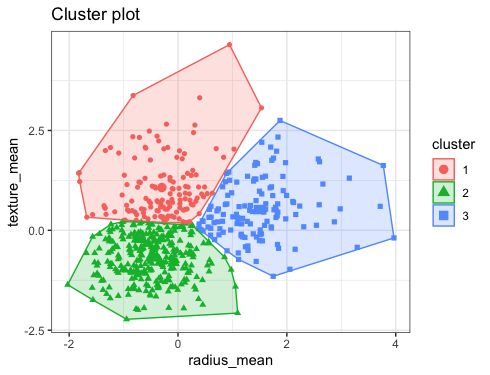
\includegraphics[width=10cm]{kmeans.png}
    \caption{Diagram demonstrating the k-means algorithm.}
    \label{fig:k-means}
\end{figure}
\subsubsection{Implementing K-means}
The algorithm is relatively straightforward to code as many libraries already have them embedded within them.
The first step is to determine K.
The math behind the algorithm is relatively simple to understand within code.
Silhouette scores are used to determine which K provides the minimum amount of distance under the Euclidean Inner Product between a centroid and its surrounding points \cite{mora-clustering}.
K is the number of centroids used to cluster the points.
The code determines the silhouette score for the first 5 values of K, and it is important to do a reasonable amount of testing for K to find the global minimum rather than a local one.
Once the values are each calculated, the value of K with the maximum silhouette score is used to determine the clustering.
\vspace{1em}

The next step is the actual K-means algorithm.
In terms of coding the algorithm, the value of K determined from the maximum silhouette score is used, and the code displayed below clusters the data.
The library used, Scipy, already has a kmeans function included. 
 \begin{figure}[H]
    \centering
    \begin{lstlisting}[language=Python]
import pandas as pd
from scipy.cluster.vq import vq, kmeans, whiten
import numpy as np

gps = pd.read_csv("data/interim/with-gps.csv")
coords = []
for idx, row in gps.iterrows():
    lat = row["latitude"]
    lon = row["longitude"]
    pair = []
    pair.append(lon) # x axis
    pair.append(lat) # y axis
    coords.append(pair)

coords_np = np.array(coords)

# Whiten (i.e. normalize) data
whitened = whiten(coords_np)

# Find 3 clusters in the data
codebook, distort = kmeans(whitened, 3)
# codebook is list of cluster centroids, distort is additional data
    \end{lstlisting}
    \caption{Code displaying the algorithm to implement K-means clustering.}
    \label{fig:k-means-code2}
\end{figure}
\subsubsection{Problem with K-means Algorithm}
It is important to consider that certain initial data points will cause divergent results that converge to certain points not normally"centroids." To avoid the initial value problems, we can implement k-means seeding. This simply imvolved the use of various initial values to determine which centroids are the most common ones and thus have the best convergence for the data set.
\subsubsection{Determining K: Silhouette Scores}
Determining K subjectively can cause many issues primarily in the fact that determining the optimal number for K can be deceiving and just unknown based on how chaotic the points are. 

Silhouette scores try to avoid this by determining if a certain number of points fits well for a given cluster and terribly for a neighboring cluster. There are 2 primary measurements: a(i) and b(i). a(i) is a measure of how far a given observation is from a certain cluster compared to other observations. This involves the summations of all possible distances of observations to others via the Euclidean Inner Product for distance given by the following:

\begin{equation}
a(i)=\frac{1}{|C_i|-1}\sum_{j\epsilon C_i, i\neq j}d(i,j) 
\end{equation}

b(i), on the other hand, focuses on the calculations of average distance compared to all other neighboring clusters based on the Euclidean inner product for distance.  The average distance a given observation is compared to this neighboring cluster has the following formula: 
\begin{equation}
b(i)=\min_{k\neq i}\frac{1}{|C_k|}\sum_{j\epsilon C_k}d(i,j)
\end{equation}

where $C_i$ is the set of data points. Using b(i) and a(i), the silhouette score can be expressed as the following:
\begin{equation}
s(i)=\frac{b(i)-a(i)}{max\{a(i),b(i)\}}, if |C_i|>1
\end{equation}

This score is between -1 and 1 with the one with overall higher score indicating a better fit for K. However, to counteract the problem of picking the right initial centroids, multiple calculations are done for multiple samples for a given K, then averaged. Plotting each K will show the maximum value s(i) that maximizes K.

\subsection{Gradient Boosting}
Gradient boosting is a useful algorithm when it comes to predicting data from a given data set which has many uses primarily in the field of machine learning \cite{mora-gradient-boosting}. Gradient boosting is an iterative process that continues to refine its learning process based on given "weak learners." The final goal is to essentially minimize the loss function constructed by the developer. From initial guesses, the algorithm "nudges" the value of the actual value to a point where the residual is minimized.The steps are as follows:
\begin{enumerate}
    \item Define an arbitrary differentiable loss function L(y,$\hat{y}$) where y is the true value of the data and $\hat{y}$ is the predicted value.
    \item Define $F_1(x)=\overline{y}$
    \item Determing $\hat{r}_{1i}=\frac{-dL(y_i,\hat{y_i})}{d\hat{y_1}}$ evaluated at $\hat{y_i}=F_1(x_i)$ for all N data points i=1,2,...,N
    \item a new weak learner is defined $f_2(x)$ where $\hat{r_1}~x$
    \item \[\hat{\gamma_2}=\arg\min_{\gamma}(\sum_{i=1}^{N}L(y_i,f_1(x_i)+f_2(x_i)))\]
    \item let $F_2(x)=f_1(x)+\hat{\gamma_2}f_2(x)$
    \item repeat beginning at step 3
\end{enumerate}
Another way to understand gradient boosting is by the following: 
 \begin{figure}[H]
    \centering
    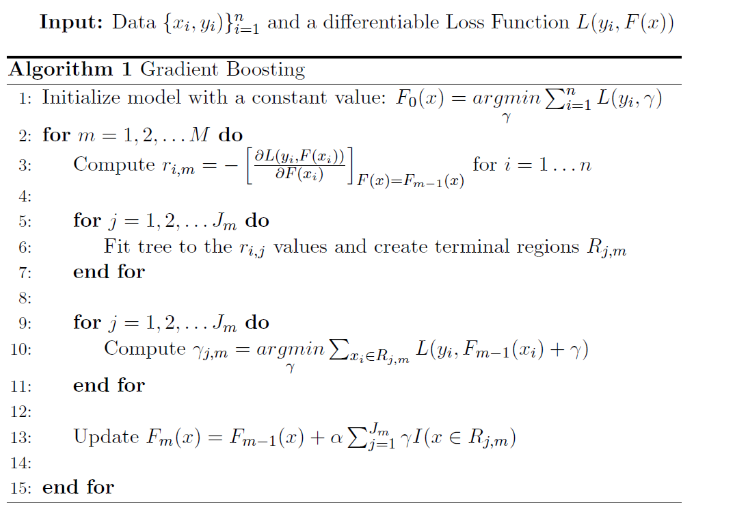
\includegraphics[width=15cm]{GBoost.png}
    \caption{Gradient Boosting Algorithm}
    \label{fig:grad-boost}
\end{figure}

In this algorithm, there are a few important variables to note. The learning rate defines how fast the adjustment occurs to determine the minimum of the loss function. A low learning rate indicates a slow process from the original first guess. A high learning rate causes the algorithm to become too inconsistent and jump all over the predictions. This trade off is important to determine a fast but consistent learning rate. 
The number of trees is also an important factor based on how much the data sparses itself. The number of trees essentially defines how many times the process iterates itself.This corresponds to the learning rate in that a higher learning rate requires less trees whereas a lower learning rate requires more trees for the loss function to minimize itself.
In this algorithm, there were M trees and J terminal leaves with n observations (or data points). Terminal leaves are the final leaves of the tree model. F represents $\hat{y}$ and R is the region the terminal tree is located in.
\subsubsection{Implementing Gradient Boosting}
We will be using scikit-learn to implement the algorithm.
The code below displays a gradient boosting algorithm where a negative mean squared error is used as the loss function.
GridSearchCV algorithm then determines the optimal hyperparameters.
 \begin{figure}[H]
    \centering
    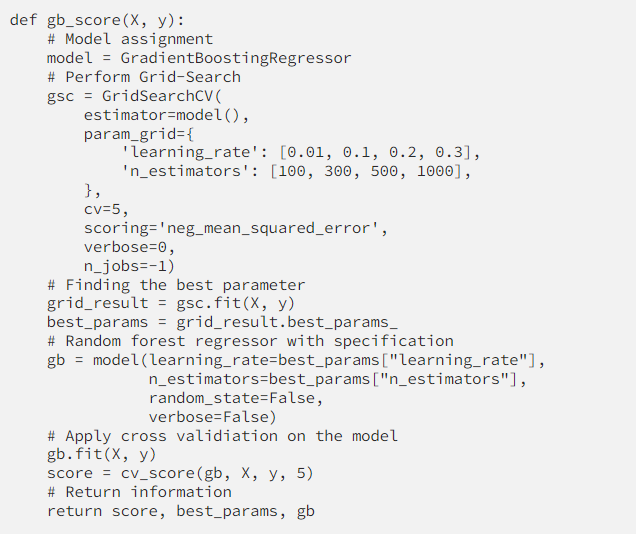
\includegraphics[width=15cm]{GBoost1.png}
    \caption{Code displaying the algorithm to implement Gradient Boosting}
    \label{fig:k-means-code2}
\end{figure}
With the negative mean squared error, the square root of the negative values are taken as the loss function provides negative values. This allows for square roots to have the real values to define the score.
 \begin{figure}[H]
    \centering
    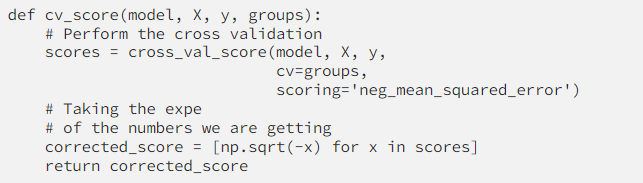
\includegraphics[width=15cm]{GBoost2.png}
    \caption{Code displaying the algorithm to implement the negative root mean squared error loss function.}
    \label{fig:k-means-code2}
\end{figure}
\subsubsection{Hyperparameter Tuning}
It is important to use the GridSearchCV algorithm so that the hyperparameters can be optimized based on the number of trees and depth used from the Random Forest.
Gradient Boosting typically is worse for smaller learning rates with higher number of trees allowing more data to fit.
Thus, a higher number of trees and learning rate overall improves the algorithm itself.
\vspace{1em}
%\subsection{Modelling}

Using all of these algorithms listed above, the final modeling of variables in real estate can be done.
At a high level this can be used to assess the importance of each variable that can affect pricing in real estate.




\section{Model Prediction}
Our first step in creating a model for the Arizona housing market was to separate the data into regions.
To do so, we converted the zipcode for each house into latitude and longitude and whitened this data.
Then, using the latitude and longitude data we conducted k-means clustering in order to separate the data into North AZ, Central AZ, and South AZ.
In the pandas dataframe, these are represented as 0, 1, and 2 respectively.
\begin{figure}[H]
    \centering
    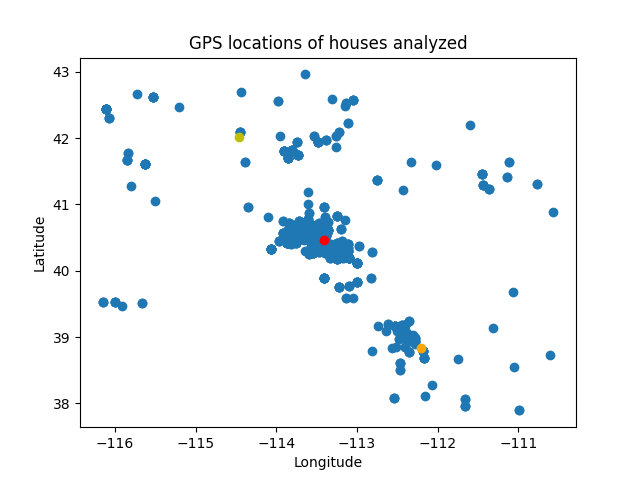
\includegraphics[width=15.5cm]{clusters.png}
    \caption{Location of the three clusters. Yellow is North AZ, red is Central AZ, and orange is South AZ.}
    \label{fig:azclusters}
\end{figure}
We then calculated the distance from each house to each cluster in order to assign them to their respective regions.
\begin{figure}[H]
    \centering
    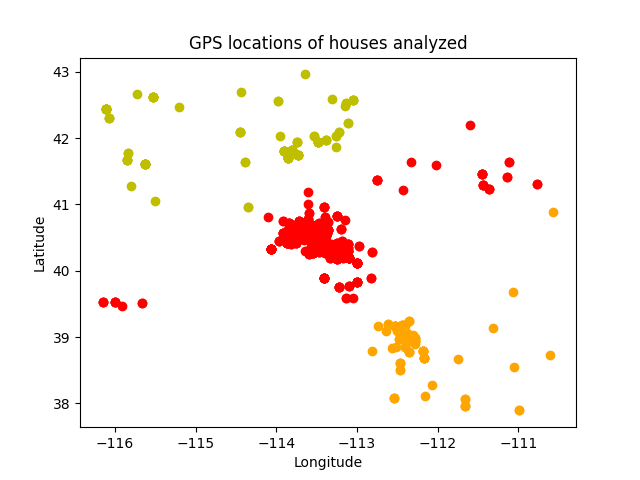
\includegraphics[width=15cm]{regions.png}
    \caption{Houses categorized into regions. Yellow is North AZ, red is Central AZ, and orange is South AZ.}
    \label{fig:azregions}
\end{figure}
We also assigned each house its city index (e.g., Phoenix has index 0), which is dependent on what city the house is located in.
City indices were determined by how expensive it is to live in a given city.
The code for making this distinction can be seen below:
 \begin{figure}[H]
    \centering
    \begin{lstlisting}[language=Python]
import pandas as pd

# order cities by how expensive they are
raw = pd.read_csv("data/processed/cleaned-final.csv")
grouped = raw.groupby('Local_area').sum().reset_index()
total = grouped.sort_values('Price', ascending=False)

cities = []
for idx, row in total.iterrows():
    if row["Local_area"] not in cities:
        cities.append(row["Local_area"])

# assign cities their indices
city_idx = []
for i in range(len(raw)):
    city_idx.append(0)

def get_city_idx(name):
    i = 0
    for city in cities:
        if name == city:
            return i
        else:
            i += 1
    return i

# assign city indices to each row
raw["city_index"] = city_idx
for idx, row in raw.iterrows():
    raw.at[idx, "city_index"] = get_city_idx(row["Local_area"])

# save data
raw.to_csv("data/processed/final-final.csv")

    \end{lstlisting}
    \caption{Determining city index by how expensive a city is}
    \label{fig:cityidx}
\end{figure}
Once each house was categorized and given a city index, we then used Gradient Boosting to make a prediction.
First we separated the data into training and test groups, which are split 85\% and 15\% respectively.
Then we used GridSearchCV to determine the optimal number of trees and learning rate for Gradient Boosting.
Once these values were determined, the training data was used to fit the model.
\section{Discussion}
In order to validate the model, the mean absolute percent error (MAPE) was calculated by
\begin{equation}
MAPE(X) = 100\times\frac{|p(X)-a(X)|}{a(X)}
\end{equation}
Where $X$ is the matrix of features for a given house, $p(X)$ is the predicted price for $X$, and $a(X)$ is the actual price for $X$.
The statistics summary for the 85 test values is shown below.
This number tells us how far off the predicted price was from the actual price.
\begin{figure}[H]
\centering
\begin{tabular}{|c|c|c|c|c|c|c|}
\hline
Mean & Std. Dev & Minimum & 1st Quartile & Median & 3rd Quartile & Maximum \\
\hline
62.870 & 155.192 & 0.420 & 12.739 & 23.304 & 41.344 & 1333.732 \\
\hline
\end{tabular}
\caption{Table showing the mean absolute percent error statistics}
\label{tab:uwu}
\end{figure}
Our median MAPE was 23\%, i.e. the median of the mean absolute percent error is 23\%.
The average MAPE was 63\%.
\begin{figure}[H]
    \centering
    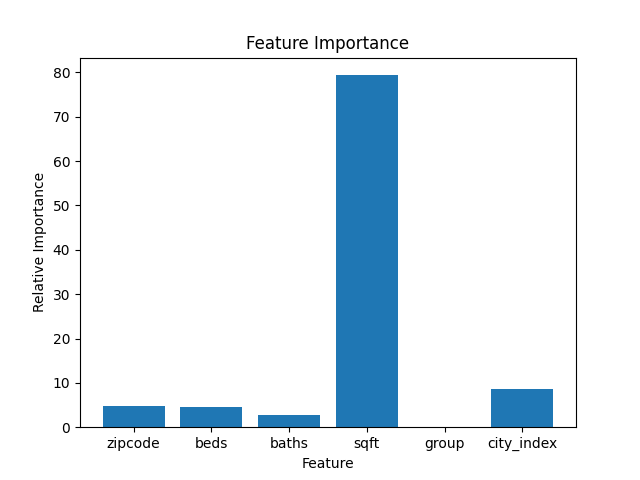
\includegraphics[width=15cm]{featureimportance.png}
    \caption{Feature importance for fitting the model.}
    \label{fig:featureimportance}
\end{figure}
Figure \label{fig:featureimportance} shows the relative importance of each feature used to fit the model.
This shows that square feet has the most importance when it comes to pricing houses, and the group (i.e. north/central/south AZ) has no relevance.
\vspace{1em}

One way the results could've been more accurate was by increasing the amount of test data.
We were using 562 out of the 563 rows from the original data set, and of those 562 only 85\% was used to train the model.
This could be accomplished by scraping Zillow for more houses.
Although we would need to clean up the data, this would allow us to create a more accurate prediction model.

Another way to obtain more accurate results would be to focus on a specific region.
We conducted analysis on all parts of the state, but focusing on a specific area (such as Maricopa county) would reduce variance in the data.
\subsection*{Conflict of Interest}
The authors declare that they have no conflict of interest.

\printbibliography

\end{document}
